%\documentclass[handout]{beamer}
\documentclass{beamer}
%\documentclass[presentation]{beamer}

\usecolortheme{Imperial}
 
\usepackage[utf8]{inputenc}
\usepackage[UKenglish]{babel}
\usepackage{booktabs}
\usepackage{caption}
\usepackage{subcaption}
\usepackage{graphicx}
\usepackage{amsmath}
\usepackage{amsfonts}
\usepackage{amssymb}
\usepackage{epstopdf}

% complying UK date format, i.e. 1 January 2001
%\usepackage{datetime}
%\let\dateUKenglish\relax
%\newdateformat{dateUKenglish}{\THEDAY~\monthname[\THEMONTH] \THEYEAR}

% Imperial College Logo, not to be changed!
\institute{
\includegraphics[height=0.7cm]{Imperial_1_Pantone_solid.eps}}

% -----------------------------------------------------------------------------


%Information to be included in the title page:
\title{Probability theory}

\subtitle{\url{https://bitbucket.org/mfumagal/statistical_inference}}

\author{Matteo Fumagalli}

\date{\today}

\begin{document}
 
\frame{\titlepage}

\begin{frame}
	\frametitle{Intended Learning Outcomes}
	By the end of this session, you will be able to:
	\begin{itemize}
		\item Describe the principles of set theory and set operations
		\item Illustrate the axiomatic foundations of probability theory and appropriate counting methods
		\item Identify dependence and indepedence of events
		\item Show the utility of distribution functions for random variables
		\item Demonstrate how to implement basic probability calculus in \texttt{R}
	\end{itemize}
\end{frame}

\begin{frame}
	\frametitle{Set theory}

	Draw conclusions about a population of objects after an experiment. What are the possible outcomes of the experiment?

	\begin{block}{Sample space}
	The set $S$ of all possible outcomes of a particular experiment is called 
	the \textit{sample space} for the experiment.
	\end{block}

\end{frame}

\begin{frame}
	\frametitle{Set theory}

	Examples of experiments:
	\begin{itemize}
		\item tossing a con: $S=\{H,T\}$
		\item GCSE scores of randomly selected pupils: \pause $S=\{0,1,2,...,8,9\}$.
		\item reaction time to a stimulus: \pause $S=(0,\infty)$.
	\end{itemize}

\end{frame}
 
\begin{frame}
	\frametitle{Set theory}

	\textcolor{red}{jupyter notebook:}

	\begin{itemize}
		\item Imagine that our experiment consists on observing the nucleotidic sequence of a particular gene of interest. What is the sample space $S_G=?$
		\item Now suppose that we are interested in making inference on the amino acidic sequence of a protein. What is the sample space $S_P=?$
		\item Suppose that our observations consist in the divergence between orthologous genes of arbitrary length. What is the sample space for such divergence $S_D=?$
	\end{itemize}

\end{frame}

\begin{frame}
	\frametitle{Sets and events}

	One the sample space has been defined (e.g. countable?), we consider collections of possible outcomes of an experiments.
	\begin{block}{Event}
		An \textit{event} is any collection of possible outcomes of an experiment, that is, any subset of $S$, including $S$ itself.
	\end{block}

	Let $A$ ben an event, a subset of $S$. We say that the event $A$ occurs if the outcome of the experiment is in the set $A$.
	\begin{equation*}
		A \subset B \iff x \in A \implies x \in B
	\end{equation*}
	\begin{equation*}
		A = B \iff A \subset B \text{ and } B \subset A
	\end{equation*}	

\end{frame}

\begin{frame}
	\frametitle{Set operations}

	Given any two events $A$ and $B$:
	\begin{itemize}
		\item Union: the union of $A$ and $B$ is the set of elements that belong to either $A$ or $B$ or both:
		\begin{equation*}
			A \cup B = \{x: x \in A \text{ or } x \in B\}
		\end{equation*}
		\pause
		\item Intersection: the intersection of $A$ and $B$ is the set of elements that belong to both $A$ and $B$:
		\begin{equation*}
			A \cap B = \{x: x \in A \text{ and } x \in B\}
		\end{equation*}
		\pause
		\item Complementation: the complement of $A$ is the set of all elements that are not in $A$:
		\begin{equation*}
			A^c = \{x:x \notin A\}
		\end{equation*}
	\end{itemize}

\end{frame}

\begin{frame}
        \frametitle{Set operations}

	\textcolor{red}{jupyter notebook:}

	Consider an experiment of drawing a nucleotidic base at random. The sample space is $S=\{A,C,G,T\}$ and some possible 
	events are $A=\{G,C,A\}$ and $B=\{T,G\}$.

	What is the union of $A$ and $B$? What is the intersect between $A$ and $B$? What is the complement of $A$? 
	What is the complement of the union of $A$ and $B$?

	Use Venn diagrams and R!


\end{frame}

\begin{frame}
        \frametitle{Properties of Set operations}

	\begin{itemize}
		\item Commutativity
		\begin{align*}
			A \cup B &= B \cup A \\ 
			A \cap B &= B \cap A
		\end{align*}
		\item Associativity
		\begin{align*}
			A \cup (B \cup C) &= (A \cup B) \cup C \\
			A \cap (B \cap C) &= (A \cap B) \cap C
		\end{align*}
	\end{itemize}

\end{frame}

\begin{frame}
        \frametitle{Properties of Set operations}

        \begin{itemize}
		\item Distributive laws
		\begin{align*}
			A \cap (B \cup C) &= (A \cap B) \cup (A \cap C) \\
			A \cup (B \cap C) &= (A \cup B) \cap (A \cup C)
		\end{align*}
		\item DeMorgan's laws
		\begin{align*}
			(A \cup B)^c &= A^c \cap B^c \\
			(A \cap B)^c &= A^c \cup B^c
		\end{align*}
	\end{itemize}

\end{frame}

\begin{frame}{Partition}

	\begin{block}{}
		Two events $A$ and $B$ are \textit{disjoint} (or mutually exclusive) if $A \cap B = \emptyset$.\\ 
		The events $A_1,A_2,...$ are pairwise disjoint if $A_i \cap A_j = \emptyset$ for all $i \neq j$.
	\end{block}

	\begin{block}{}
		If $A_1, A_2, ...$ are pairwise disjoint and $\bigcup_{i=0}^\infty A_i = S$, then the 
		collection $A_1, A_2, ...$ forms a \textit{partition} of S.
	\end{block}

\end{frame}

\begin{frame}{Axiomatic foundations}

	For each event $A$ in the sample space $S$ we associate a number between 0 and 1 that we call the 
	probability of A, denoted as $P(A)$. 

	\begin{block}{}
		A collection of subsets of $S$ is called a \textit{sigma algebra} (or Borel field), denoted 
		by $\mathcal{B}$, if it satisfies the following properties:
		\begin{enumerate}
			\item $\emptyset \in \mathcal{B}$
			\item if $A \in \mathcal{B}$, then $A^c \in \mathcal{B}$ 
			\item if $A_1, A_2, ... \in \mathcal{B}$, then $\bigcup_{i=1}^\infty A_i \in \mathcal{B}$
		\end{enumerate}
	\end{block}

\end{frame}

\begin{frame}{Axiomatic foundations}

	\textcolor{red}{jupyter notebook:}
	\begin{itemize}
		\item Is the collection of sets $\{\emptyset, S\}$ a sigma algebra with $S$?
		\item If $S$ has $n$ elements, there are $2^n$ sets in $\mathcal{B}$. What is $\mathcal{B}$ if $S=\{1,2,3\}$?
	\end{itemize}

\end{frame}

\begin{frame}{Probability function}

	\begin{block}{}
		Given a sample space $S$ and an associated sigma algebra $\mathcal{B}$, a \textit{probability function} is 
		a function $P$ with domain $\mathcal{B}$ that satisfies:
		\begin{enumerate}
			\item $P(A) \geq 0$ for all $A \in \mathcal{B}$
			\item $P(S)=1$
			\item If $A_1, A_2, ... \in \mathcal{B}$ are pairwise disjoint, then $P(\bigcup_{i=1}^\infty)=\sum_{i=1}^\infty P(A_i)$
		\end{enumerate}
	\end{block}
	Any function $P$ that satisfies these Axioms of Probability is called a probability function.

\end{frame}

\begin{frame}{Probability function}

	Let $S=\{s_1, s_2, ..., s_n\}$ a finite and/or countable set. 

	Let $\mathcal{B}$ be any sigma algebra of subsets of $S$. 

	Let $p_1, p_2, ..., p_n$ nonnegative numbers that sum to 1. 

	For any $A \in \mathcal{B}$, define $P(A)$ by
	\begin{equation*}
		P(A) = \sum_{\{i:s_i \in A\}} p_i
	\end{equation*}
	Then $P$ is a probability function on $\mathcal{B}$.

\end{frame}

\begin{frame}{Calculus}

	If $P$ is a probability function and $A$ is any set in $\mathcal{B}$, then
	\begin{enumerate}
		\item $P(\emptyset)=0$
		\item $P(A) \leq 1$
		\item $P(A^c) = 1 - P(A)$
	\end{enumerate}

	\vskip 1cm
	\tiny{prove nr.3?}

\end{frame}

\begin{frame}{Calculus}

	If $P$ is a probability function and $A$ and $B$ are any sets in $\mathcal{B}$, then
        \begin{enumerate}
                \item $P(B \cap A^c) = P(B) - P(A \cap B)$
                \item $P(A \cup B) = P(A) + P(B) - P(A \cap B)$
                \item if $A \subset B$, then $P(A) \leq P(B)$
        \end{enumerate}

\end{frame}

\begin{frame}{Calculus}

	Since $P(A \cup B) \leq 1$, then
	\begin{equation*}
		P(A \cap B) \geq P(A) + P(B) - 1
	\end{equation*}
	
	This is a special case of the \textit{Bonferroni's Inequality}: to bound the probability of a simultaneous 
	event from the probabilities of the individual events.

\end{frame}

\begin{frame}{Calculus}

	If $P$ is a probability function, then
	\begin{enumerate}
		\item $P(A) = \sum_{i=1}^\infty P(A \cap C_i)$ for any partition $C_1, C_2, ...$ of $S$
		\item $P(\bigcup_{i=1}^\infty A_i) \leq \sum_{i=1}^\infty P(A_i) $ for any sets $A_1, A_2, ...$ 
	\end{enumerate}

	This property is called \textit{Boole's Inequality}, a general version of the Bonferroni's Inequality.

\end{frame}

\begin{frame}{Counting}

	Methods of counting are used to construct probability assignments on finite sample spaces.

	\begin{block}{Fundamental Theorem of Counting}
		If a job consists of $k$ separate tasks, the $i-th$ of which can be done in $n_i$ ways, $i=1,...,k$, 
		then the entire job can be done in $n_1 \times n_2 \times ... \times n_k$ ways.
	\end{block}

\end{frame}

\begin{frame}{Counting}

	Let's assume that one protein domain is comprised of 6 amino acids. To be able to calculate the 
	probability of having exactly one sequence we first must count how many different combinations 
	of 6 amino acids can be observed.

	\vskip 1cm

	Is that enough information to calculate such probabilities? What else do we need?

\end{frame}

\begin{frame}{Counting}

	\begin{table}[]
		\begin{tabular}{c|c|c}
			& without replacement & with replacement \\
		\hline
			ordered &  & \\
		\hline
			unordered &  &\\
		\hline
		\end{tabular}
	\end{table}

\end{frame}

\begin{frame}{Ordered, without replacement}

	The first amino acid can be selected in ... ways, the second in ... 

	\pause
	\begin{block}{}
		For a positive integer $n$, $n!$ (read $n$ factorial) is the product of all the positive integers less than or equal to $n$, that is, $n! =  n \times (n-1) \times (n-2) \times ... \times 2 \times 1$. We define $0!=1$.
	\end{block}

\end{frame}

\begin{frame}{Ordered, with replacement}

	All amino acids can be selected in ... ways ...

\end{frame}

\begin{frame}{Unordered, without replacement}

	Since we know the number of ways when the ordering must be taken into account, ..., we need to ... this number by all the possible ways that 6 amino acid can be ordered, which is ...

	\pause

	\begin{block}{}
		For nonnegative integers $n$ and $r$, where $n \geq r$, we define the 
		symbol ${n \choose r}$, read $n \text{ choose } r$, as
		\begin{equation*}
			{n \choose r} = \frac{n!}{r!(n-r)!}
		\end{equation*}
	\end{block}
	These numbers are also called \textit{binomial coefficients}.

\end{frame}

\begin{frame}{Unordered, with replacement}

	Imagine to assign 6 amino acids on the 20 possible values. We can reduce the ways of counting noting that we just need to keep track of the arrangement and that the two boundaries of the 22 interval bounds (since we can 20 bins) are not relevant. Therefore, we have $\frac{25!}{6!19!}$ ways.

	${n+r-1} \choose {r}$

	\vskip 1cm

	\textcolor{red}{jupyter notebook:}
	fill in the table of counting methods.

\end{frame}

\begin{frame}{Enumerating outcomes}

	Suppose $S=\{s_1,...,s_n\}$ is a finite sample space. If all the outcomes are equally likely, then $P(\{s_i\})=1/N$ for every outcome $s_i$. 

	If so,
	\begin{equation*}
		P(A) = \sum_{s_i \in A} P(\{s_i\}) = \sum_{s_i \in A} \frac{1}{N} = \frac{\text{nr. elements in } A}{\text{nr. elements in } S}
	\end{equation*}


\end{frame}

\begin{frame}{Conditional probability}

	\begin{block}{}
		If $A$ and $B$ are events in $S$, and $P(B)>0$, then the \textit{conditional probability of A given B}, 
		written $P(A|B)$, is
		\begin{equation*}
			P(A|B) = \frac{P(A \cap B)}{P(B)}
		\end{equation*}
	\end{block}

	\pause
	The original sample space $S$ has been \textbf{updated} to $B$, so that $P(B|B)=1$.

	If $A$ and $B$ are disjoints, then $P(A \cap B)=0$ and $P(A|B)=P(B|A)=0$.

\end{frame}

\begin{frame}{Independence}

	\begin{block}{}
		Two events, $A$ and $B$, are statistically independent if
		\begin{equation*}
			P(A \cap B) = P(A)P(B)
		\end{equation*}
	\end{block}

	If the occurrence of $B$ has no effect on the probability of $A$, then $P(A|B)=P(A)$.

\end{frame}

\begin{frame}{Independence}

	If $A$ and $B$ are independent events, then the following pairs are also independent:
	\begin{itemize}
		\item $A$ and $B^c$
		\item $A^c$ and $B$
		\item $A^c$ and $B^c$
	\end{itemize}

\end{frame}

\begin{frame}{Independence}

	\begin{block}{}
		A collection of events $A_1, A_2, ..., A_n$ are \textit{mutually independent} if for any
		subcollection $A_{i_1},...,A_{i_k}$, we have
		\begin{equation*}
			P(\bigcap_{j=1}^k A_{i_j} ) = \prod_{j=1}^k P(A_{i_j})
		\end{equation*}
	\end{block}

	Simultaneous independence requires a strong definition.

\end{frame}

\begin{frame}{Random variables}

	Assume we are interested in the GC content of a nucleotidic sequence $\{A,C,G,T\}$ of 50 base pairs.

	If we record "1" for a GC base and "0" otherwise (A or T), what is the sample space for this experiment?

	\pause

	$S$ has $2^{50}$ elements!

\end{frame}

\begin{frame}{Random variables}

        Assume we are interested in the GC content of a nucleotidic sequence $\{A,C,G,T\}$ of 50 base pairs.
        We record "1" for a GC base and "0" otherwise (A or T), 

	If we define $X$ = number of 1s recorded out of 50, what is the sample space for $X$?

        \pause

        $S$ for $X$ is the set of integers $\{0,1,2,...,50\}$!

\end{frame}

\begin{frame}{Random variables}

	When we define $X$, we created a mapping (a function) from the original sample space to a new sample space.
	\begin{block}{}
		A \textit{random variable} is a function from a sample space $S$ into the real numbers.
	\end{block}

	In defining a random variable, we also define a new sample space. 
	Can our probability function on the original sample space be used for the random variable?

\end{frame}

\begin{frame}{Random variables}

	Suppose we have a sample space $S=\{s_1,...,s_n\}$ with a probability function $P$ and we 
	define a random variable $X$ with range $\mathcal{X}=\{x_1,...,x_m\}$.

	\begin{equation*}
		P_X(X=x_i) =  P(\{s_j \in S : X(s_j)=x_i\} )
	\end{equation*}

	If $\mathcal{X}$ is uncountable?
	\pause
	\begin{equation*}
		P_X(X \in A) =  P(\{s \in S : X(s) \in A\} )
	\end{equation*}

\end{frame}

\begin{frame}{Distribution functions}

With every random variable $X$, we associate a function called the cumulative distribution function of $X$.

	\begin{block}{}
		The \textit{cumulative distribution function} (or cdf) of a random variable $X$, 
		denoted by $F_X(x)$ is defined by
		\begin{equation*}
			F_X(x) = P_X(X \leq x) \text{, for all } x
		\end{equation*}
	\end{block}

	\vskip 1cm

	\small{Experiment: roll a die, what is $F_X(x)?$}

\end{frame}

\begin{frame}{Cumulative distribution function}

	\textcolor{red}{jupyter notebook:}

	Consider the experiment of sampling three nucleotidic bases and let $X$ be the number of GC bases observed.
	What is the cdf of $X$?

	\pause

	\begin{align*}
		F_X(x) &= 0 \text{, if } -\infty < x < 0 \\
		F_X(x) &= ? \text{, if } \\
		...
	\end{align*}

\end{frame}

\begin{frame}{Cumulative distribution function}

	The function $F_X(x)$ is a cdf if and only if:
	\begin{enumerate}
		\item $\lim_{x \rightarrow -\infty} F_X(x)=0$ and $\lim_{x \rightarrow \infty} F_X(x)=1$
		\item $F_X(x)$ is a nondecreasing function of $x$
		\item $F_X(x)$ is right-continuous
	\end{enumerate}

\end{frame}

\begin{frame}{Cumulative distribution function}

	Whether a cdf is continuous or not corresponds to the associated random variable being continuous or not.

	\begin{block}{}
		A random variable $X$ is \textit{continuous} if $F_X(x)$ is a continuous function of $x$. 
		A random variable $X$ is \textit{discrete} if $F_X(x)$ is a step function of $x$.
	\end{block}

\end{frame}

\begin{frame}{Cumulative distribution function}


	\begin{block}{}
		The random variables $X$ and $Y$ are \textit{identically distributed} if, for every set $A \in \mathcal{B}^1$ (the smallest algebra sigma), $P(X \in A) = P(Y \in A)$.
	\end{block}

	If $X$ and $Y$ are identically distributed, $F_X(x)=F_Y(x)$ for every $X$.

	$F_X(x)$ completely determines the probability distribution of a random variable $X$.

\end{frame}

\begin{frame}{Density and mass functions}

	\begin{block}{}
		The \textit{probability mass function (pmf)} of a discrete random variable $X$ is given by
		\begin{equation*}
			f_X(x) = P(X=x) \text{ for all } x
		\end{equation*}

	\end{block}

\end{frame}

\begin{frame}{Probability mass function}

	From the pmf, we can calculate probabilities of events, as 
	\begin{equation*}
		P(a \leq X \leq b) = \sum_{k=a}^b f_X(k)
	\end{equation*}
	for positive integers $a$ and $b$, with $a \leq b$.

	\vskip 1cm

	What happens if $F_X(x)$ is continuos?

\end{frame}

\begin{frame}{Probability density function}

        \begin{block}{}
		The \textit{probability density function}, (or pdf), $f_X(x)$, of a continuous random 
		variable $X$ is the function that satisfies
		\begin{equation*}
			F_X(x) = \int_{-\infty}^{x} f_X(t) dt \text{ for all } x
		\end{equation*}
        \end{block}

	\pause 

	\begin{equation*}
		\frac{d}{dx} F_X(x) = f_X(x)
	\end{equation*}

	\begin{equation*}
		P(X \leq x) = F_X(x) = \pause \int_{-\infty}^x f_x(t) dt
	\end{equation*}

\end{frame}

\begin{frame}{Probability mass/density function}

	A function $f_X(x)$ is a pdf (or pmf) of a random variable $X$ if and only if
	\begin{enumerate}
		\item $f_X(x) \geq 0$ for all $x$
		\item $\sum_x f_X(x)=1$ (pmf) or $\int_{-\infty}^{\infty} f_X(x) dx =1 $ (pdf)
	\end{enumerate}

\end{frame}

\begin{frame}{Probability distributions}

	\begin{itemize}
		\item Discrete probability distributions include: the uniform discrete, Bernoulli,
binomial, geometric and Poisson distributions.
		\item Univariate continuous probability distributions include the uniform continuous, exponential, Normal, Chi-squared ($\chi^2$), log-normal, Gamma.
	\end{itemize}

\end{frame}

\begin{frame}{Discrete uniform distribution}
	\begin{figure}
		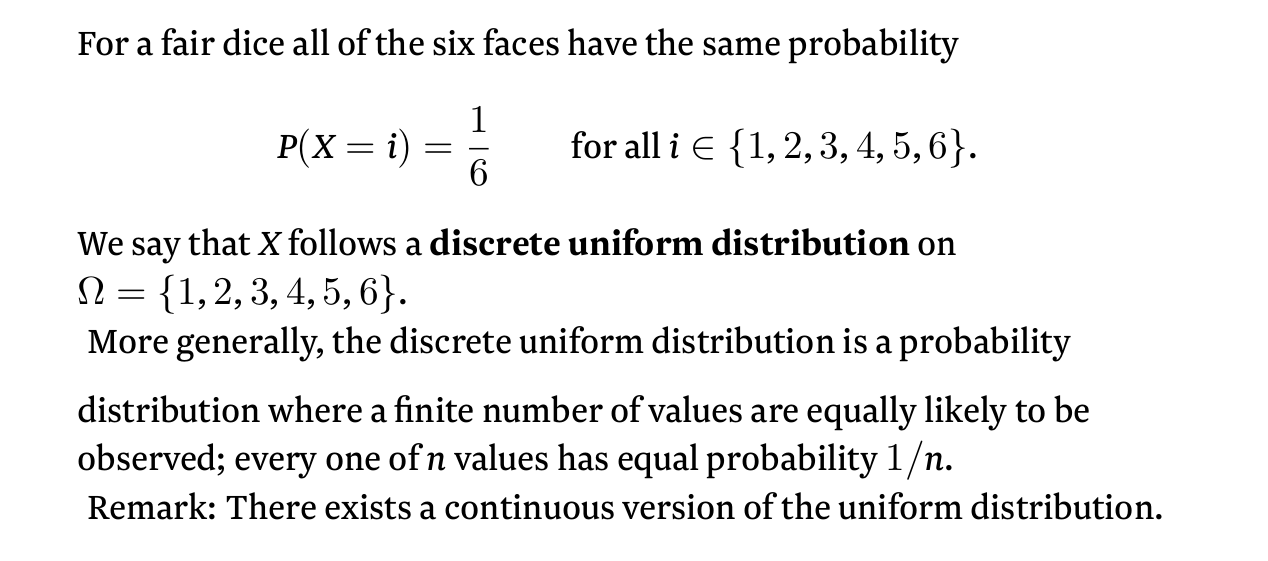
\includegraphics[width=0.9\linewidth]{uniform.png}
	\end{figure}
	What is the pmf (or pdf?) and cdf?
\end{frame}

\begin{frame}{Expectations and variance}

	The expected value of a continuous random variable $X$ is
	\begin{equation*}
		E[X] = \int_{-\infty}^{\infty} x f_X(x) dx
	\end{equation*}

	The variance of a continuous random variable is
	\begin{equation*}
		Var[X] = E[(X-E[X])^2] = E[X^2] - (E[X])^2
	\end{equation*}

\end{frame}

\begin{frame}{Bernoulli distribution}
	\begin{figure}
                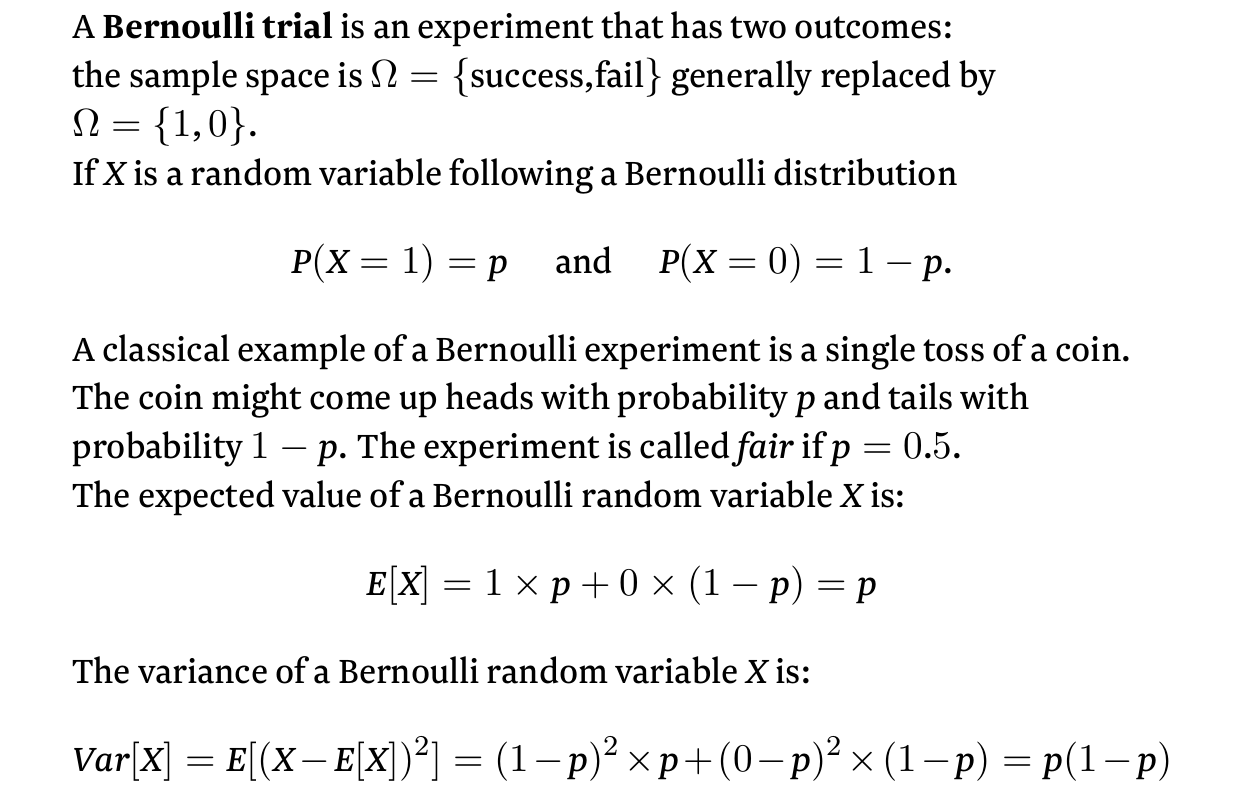
\includegraphics[width=0.9\linewidth]{bern.png}
        \end{figure}
\end{frame}

\begin{frame}{Binomial distribution}
	\begin{figure}
                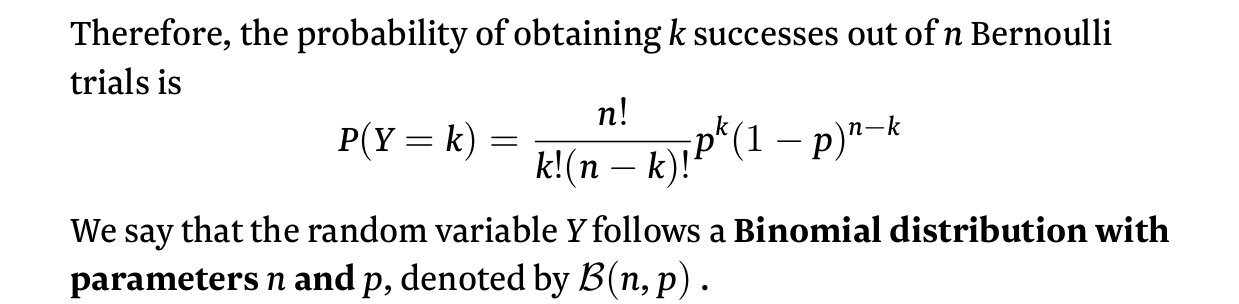
\includegraphics[width=0.9\linewidth]{binomial.png}
        \end{figure}
	$E[Y]=np$\\
	$Var[Y]=np(1-p)$

	The variance is a measure of spread and it increases with $n$ and
	decreases as $p$ approaches 0 or 1. For a given $n$, the variance is
	maximized when $p = 0.5$.

\end{frame}

\begin{frame}{Continuous - exponential distribution}
	\begin{figure}
                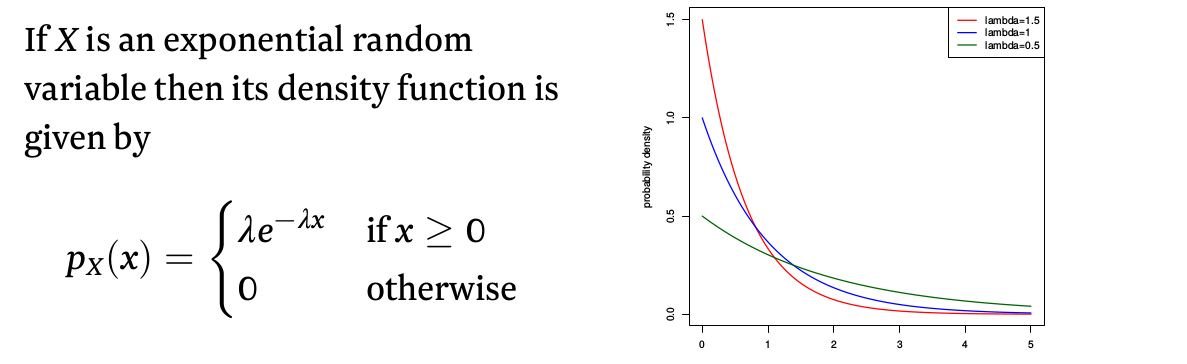
\includegraphics[width=0.9\linewidth]{exp.png}
        \end{figure}
	$E[Y]=1 / \lambda$\\
        $Var[Y]= 1 / \lambda^2$
\end{frame}

\begin{frame}{Continuous - Normal distribution}
	\begin{figure}
                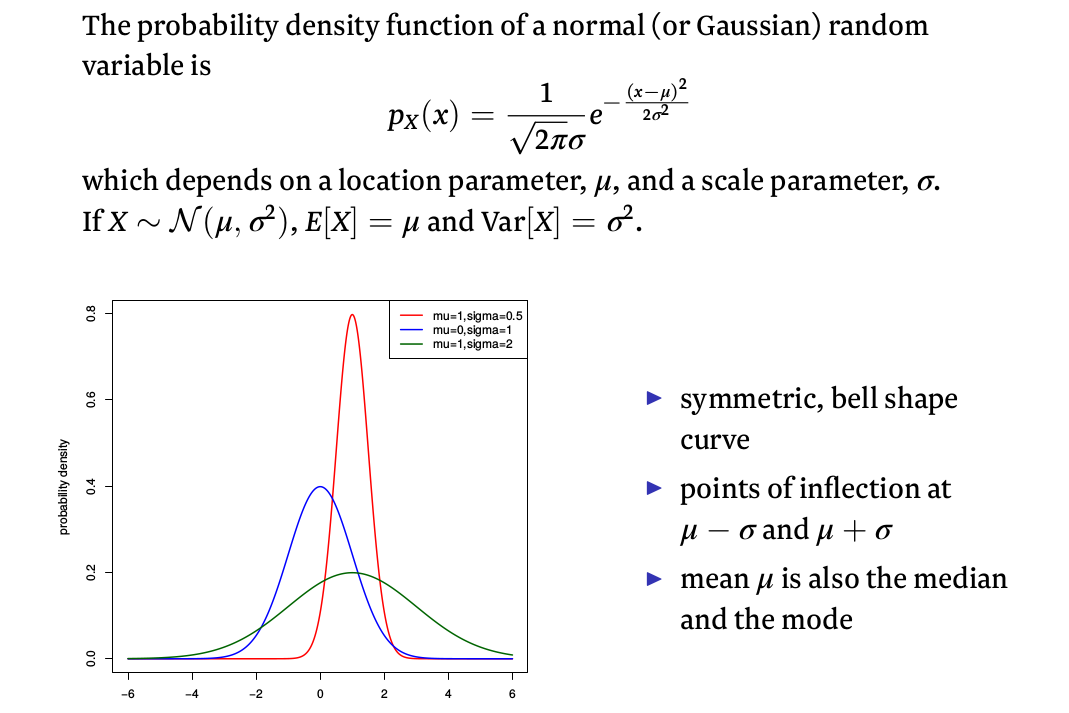
\includegraphics[width=0.8\linewidth]{normal.png}
        \end{figure}
\end{frame}

\begin{frame}{Expectations and variance}

	\begin{itemize}
		\item If $X$ is a continuous random variable with pdf $f_X(x)$, then for 
			any real-valued function $g$
			\begin{equation*}
				E[g(X)] = \int_{-\infty}^{\infty} g(x) f_X(x) dx
			\end{equation*}
		\item If $a$ and $b$ are constants, $E[aX+b]=aE[X]+b$ and $Var[aX+b]=a^2Var[X]$
	\end{itemize}

\end{frame}

\end{document}

